\subsection{Kurven, die sich berühren, Normale und Schnittwinkel}
\label{Winkel}
\subsubsection{Berühren}

% \begin{LA}
%     {Einführungsaufgaben}{}
%     \begin{enumerate}
%         \item Zeichnen Sie mit \href{https://www.geogebra.org}{Geogebra} in einem Koordinatensystem den Graphen der Funktion $f(x) = x^2-2x$ und die Gerade $t: \, y= 4x-9$. Fügen Sie die Grafik in dieses Dokument ein.
%         \item Weisen Sie nach, dass die Gerade $t$ eine Tangente an den Graphen von $f$ ist, indem Sie rechnerisch überprüfen, dass beide an der Stelle $x=3$ durch denselben Punkt verlaufen ($f(3)=t(3)$) und die gleiche Steigung haben. ($f'(3)=t'(3)$).
%         \item Berechnen Sie die Gleichung der Tangente $t_2$, welche den Graphen von $f$ an der Stelle $x=2$ berührt. Nutzen Sie dazu den Ansatz $t_2 : \, y=ax+b$ und ermitteln Sie $a$ und $b$ mit geeigneten Gleichungen.
%         \item Zeichnen Sie auch die Gerade $t_2$ mit Geogebra und überprüfen Sie so da Resultat.
%         \item Bestimmen Sie rechnerisch die Gleichung der Tangente, welche den Graphen von $g(x)= \frac{x}{x-1}$ an der Stelle $x=-1$ berührt und überprüfen Sie das Ergebnis mit Geogebra.
%         \item Geben Sie ein \glqq Rezept\grqq{} an, wie man allgemein die Gleichung der Tangente $t$ bestimmen kann, welche den Graphen einer Funktion $f$ an einer vorgegebenen Stelle $x_0$ bestimmen kann.
%     \end{enumerate} 
% \end{LA}
% \clearpage

Die Ableitung $f'(x_0)$ an einer bestimmten Stelle $x_0$ ist geometrisch gesehen die Steigung der Tangente an den Graphen der Funktion $f$. Damit haben wir schon mehrmals die Gleichung der Tangente an einen Funktionsgraphen ermittelt.
\begin{bsp}
    {Warm up}{}
    Wir betrachten als Beispiel den Graphen der Funktion $f(x)=x\cdot \ln(x) $
    \begin{center}
        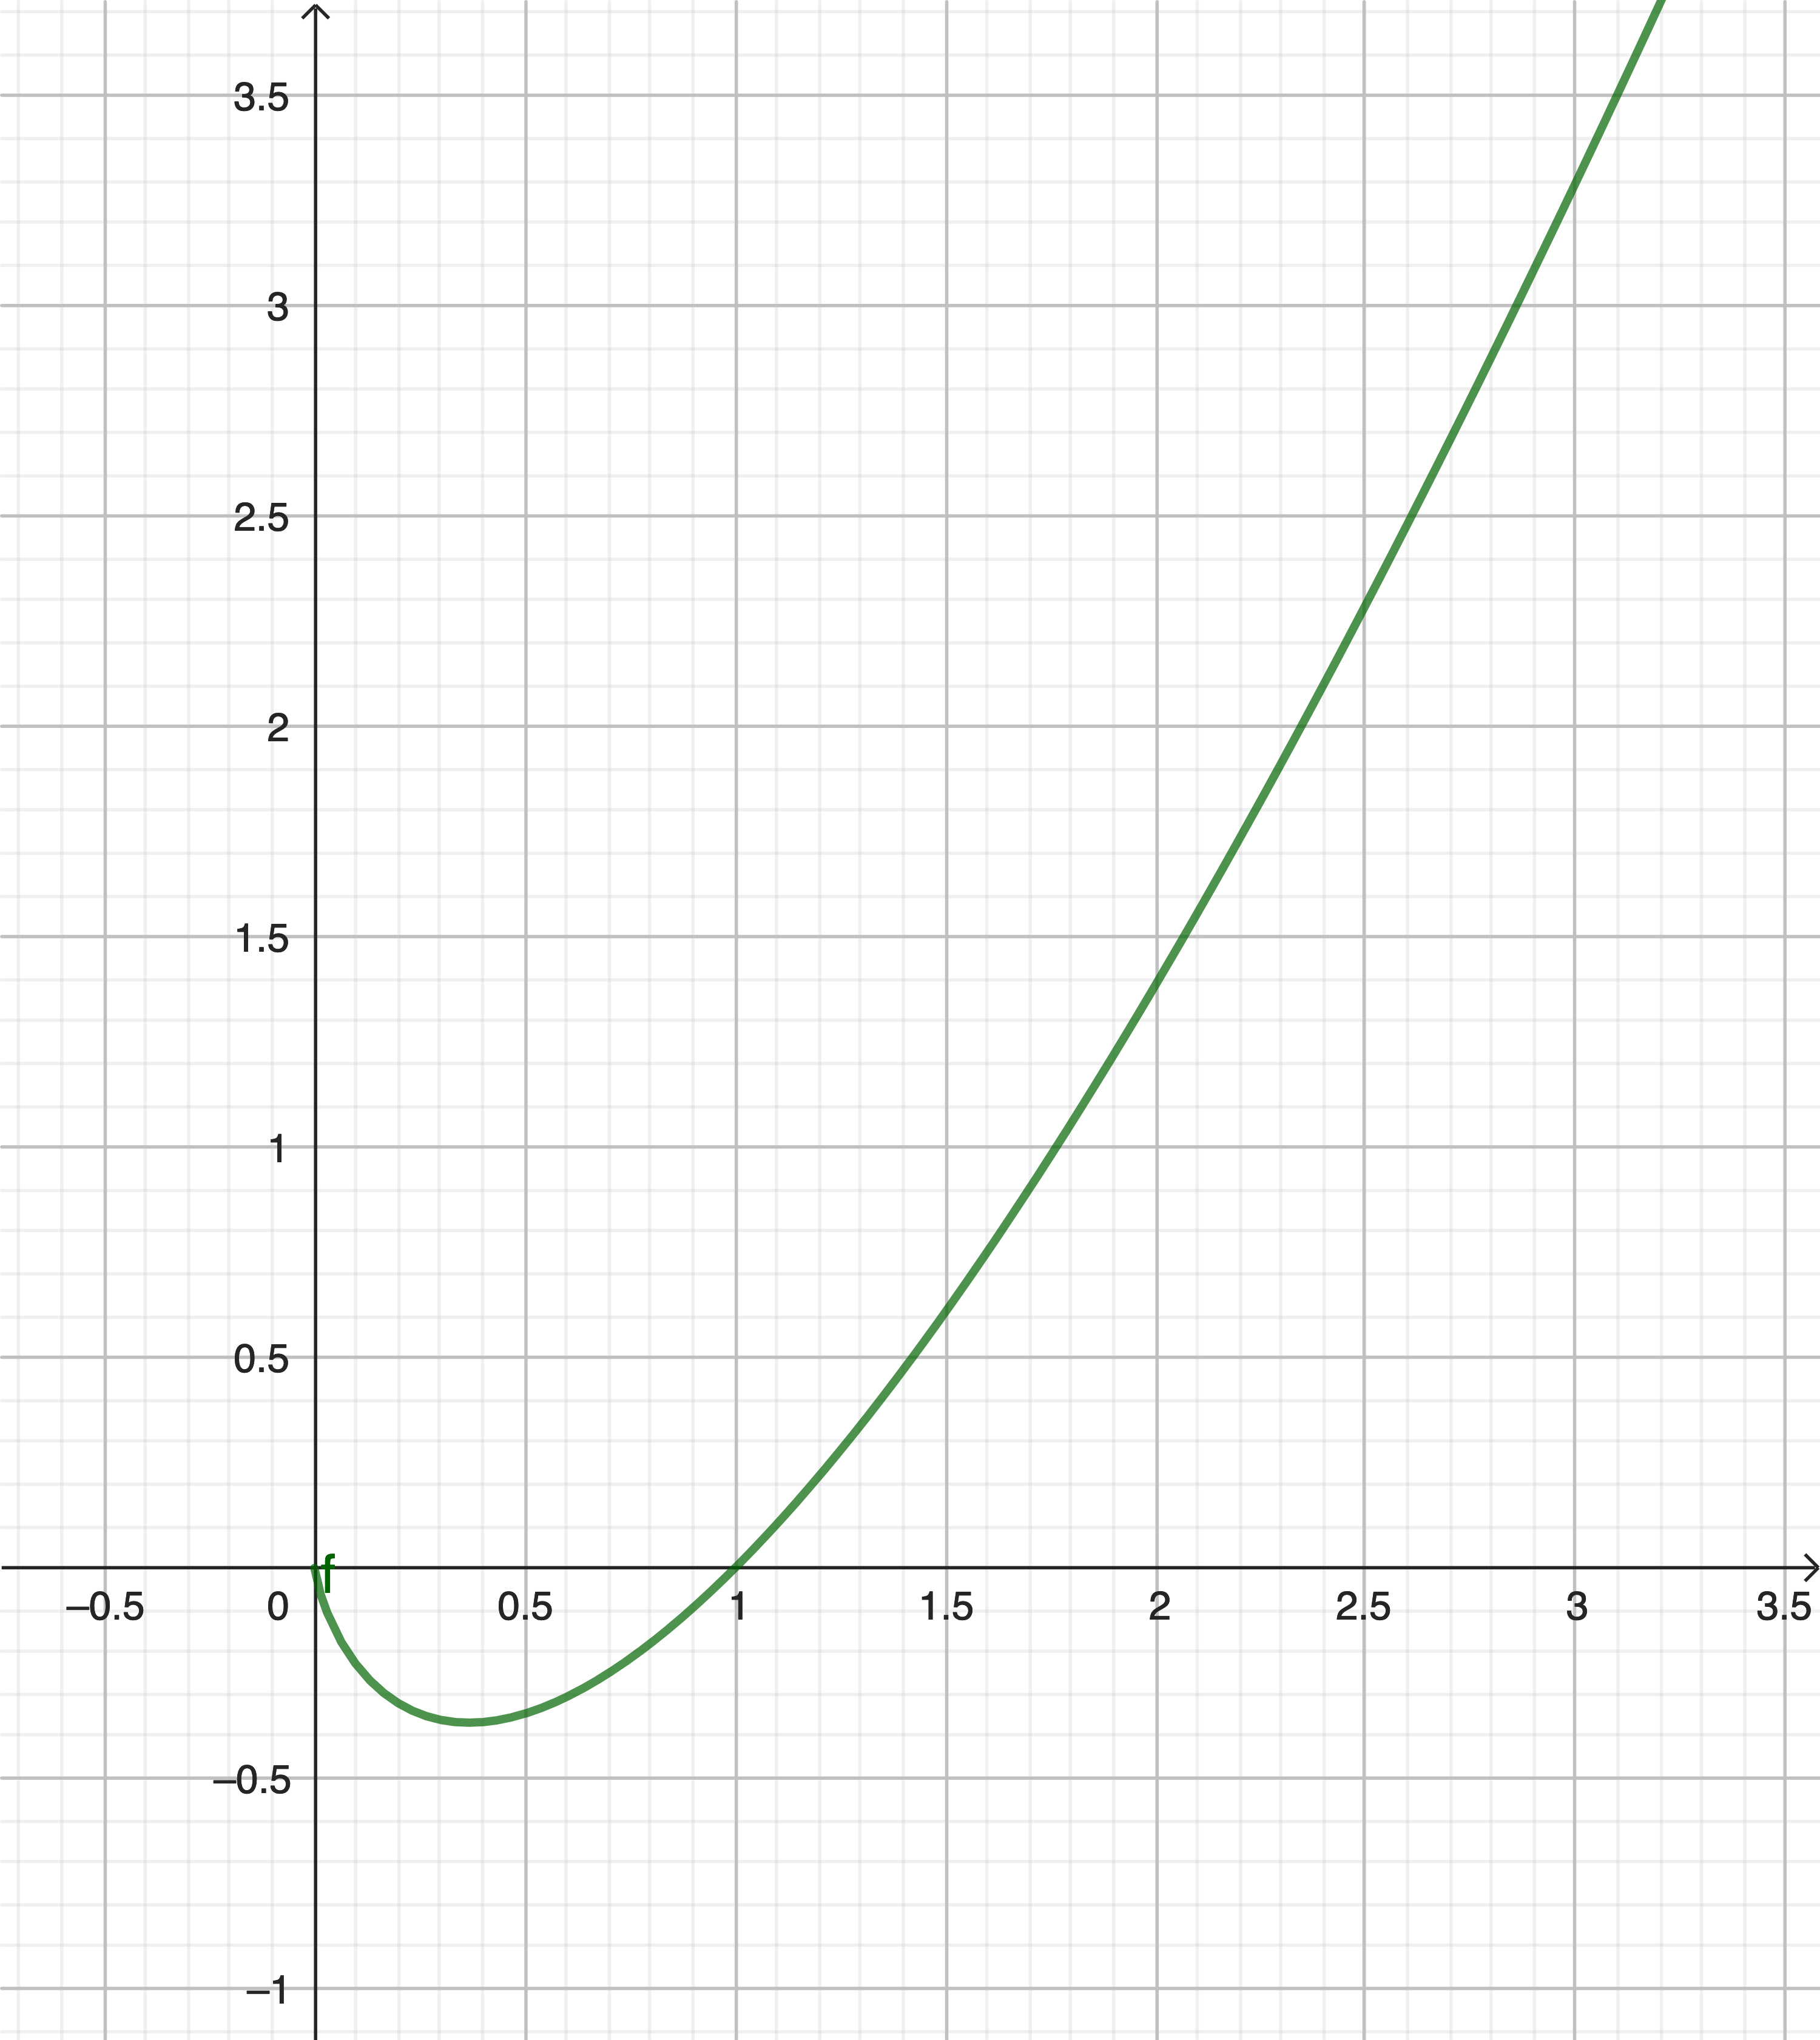
\includegraphics[scale=1]{media/xlnx.png}
    \end{center}
    Gesucht ist die Gleichung der Tangente an den Graphen an der Stelle $x=e$.
    \vspace*{10cm}
    % Ansatz: $t: \, y=ax+b$

    % An der Berührungsstelle haben Tangente und Kurve die gleiche Steigung: $a = f'(e)$ wobei $f'(x)=1\cdot \ln(x) + x\cdot \frac{1}{x}= \ln(x)+1$. Also
    % $$a=f'(e)=\ln(e)+1=2 \Longrightarrow t: \, y= 2x+b$$
    
\end{bsp}
\clearpage
\begin{satz}{Tangente an einen Funktionsgraphen}{}
    Eine Gerade $t: \, y = ax+b$ ist genau dann die Tangente an den Graphen der Funktion $f$ an der Stelle $x_0$, wenn gilt
    $$t'(x_0)=f'(x_0) \qquad \text{und} \qquad t(x_0)=f(x_0)$$

    Man sagt dann, dass die Gerade $t$ den Graphen von $f$ an der Stelle $x_0$ \emph{berührt}.
\end{satz}
Im Unterschied zu Kreistangenten oder auch Tangenten an Parabeln können Tangenten an allgemeine Funktionsgraphen auch mehrere gemeinsame Punkte mit dem dem Graphen haben. Die Gerade im Bild unten \emph{berührt} den Funktionsgraphen im Punkt $B$ und \emph{schneidet} ihn ausserdem an der Stelle $x=-1.5$
\begin{center}
    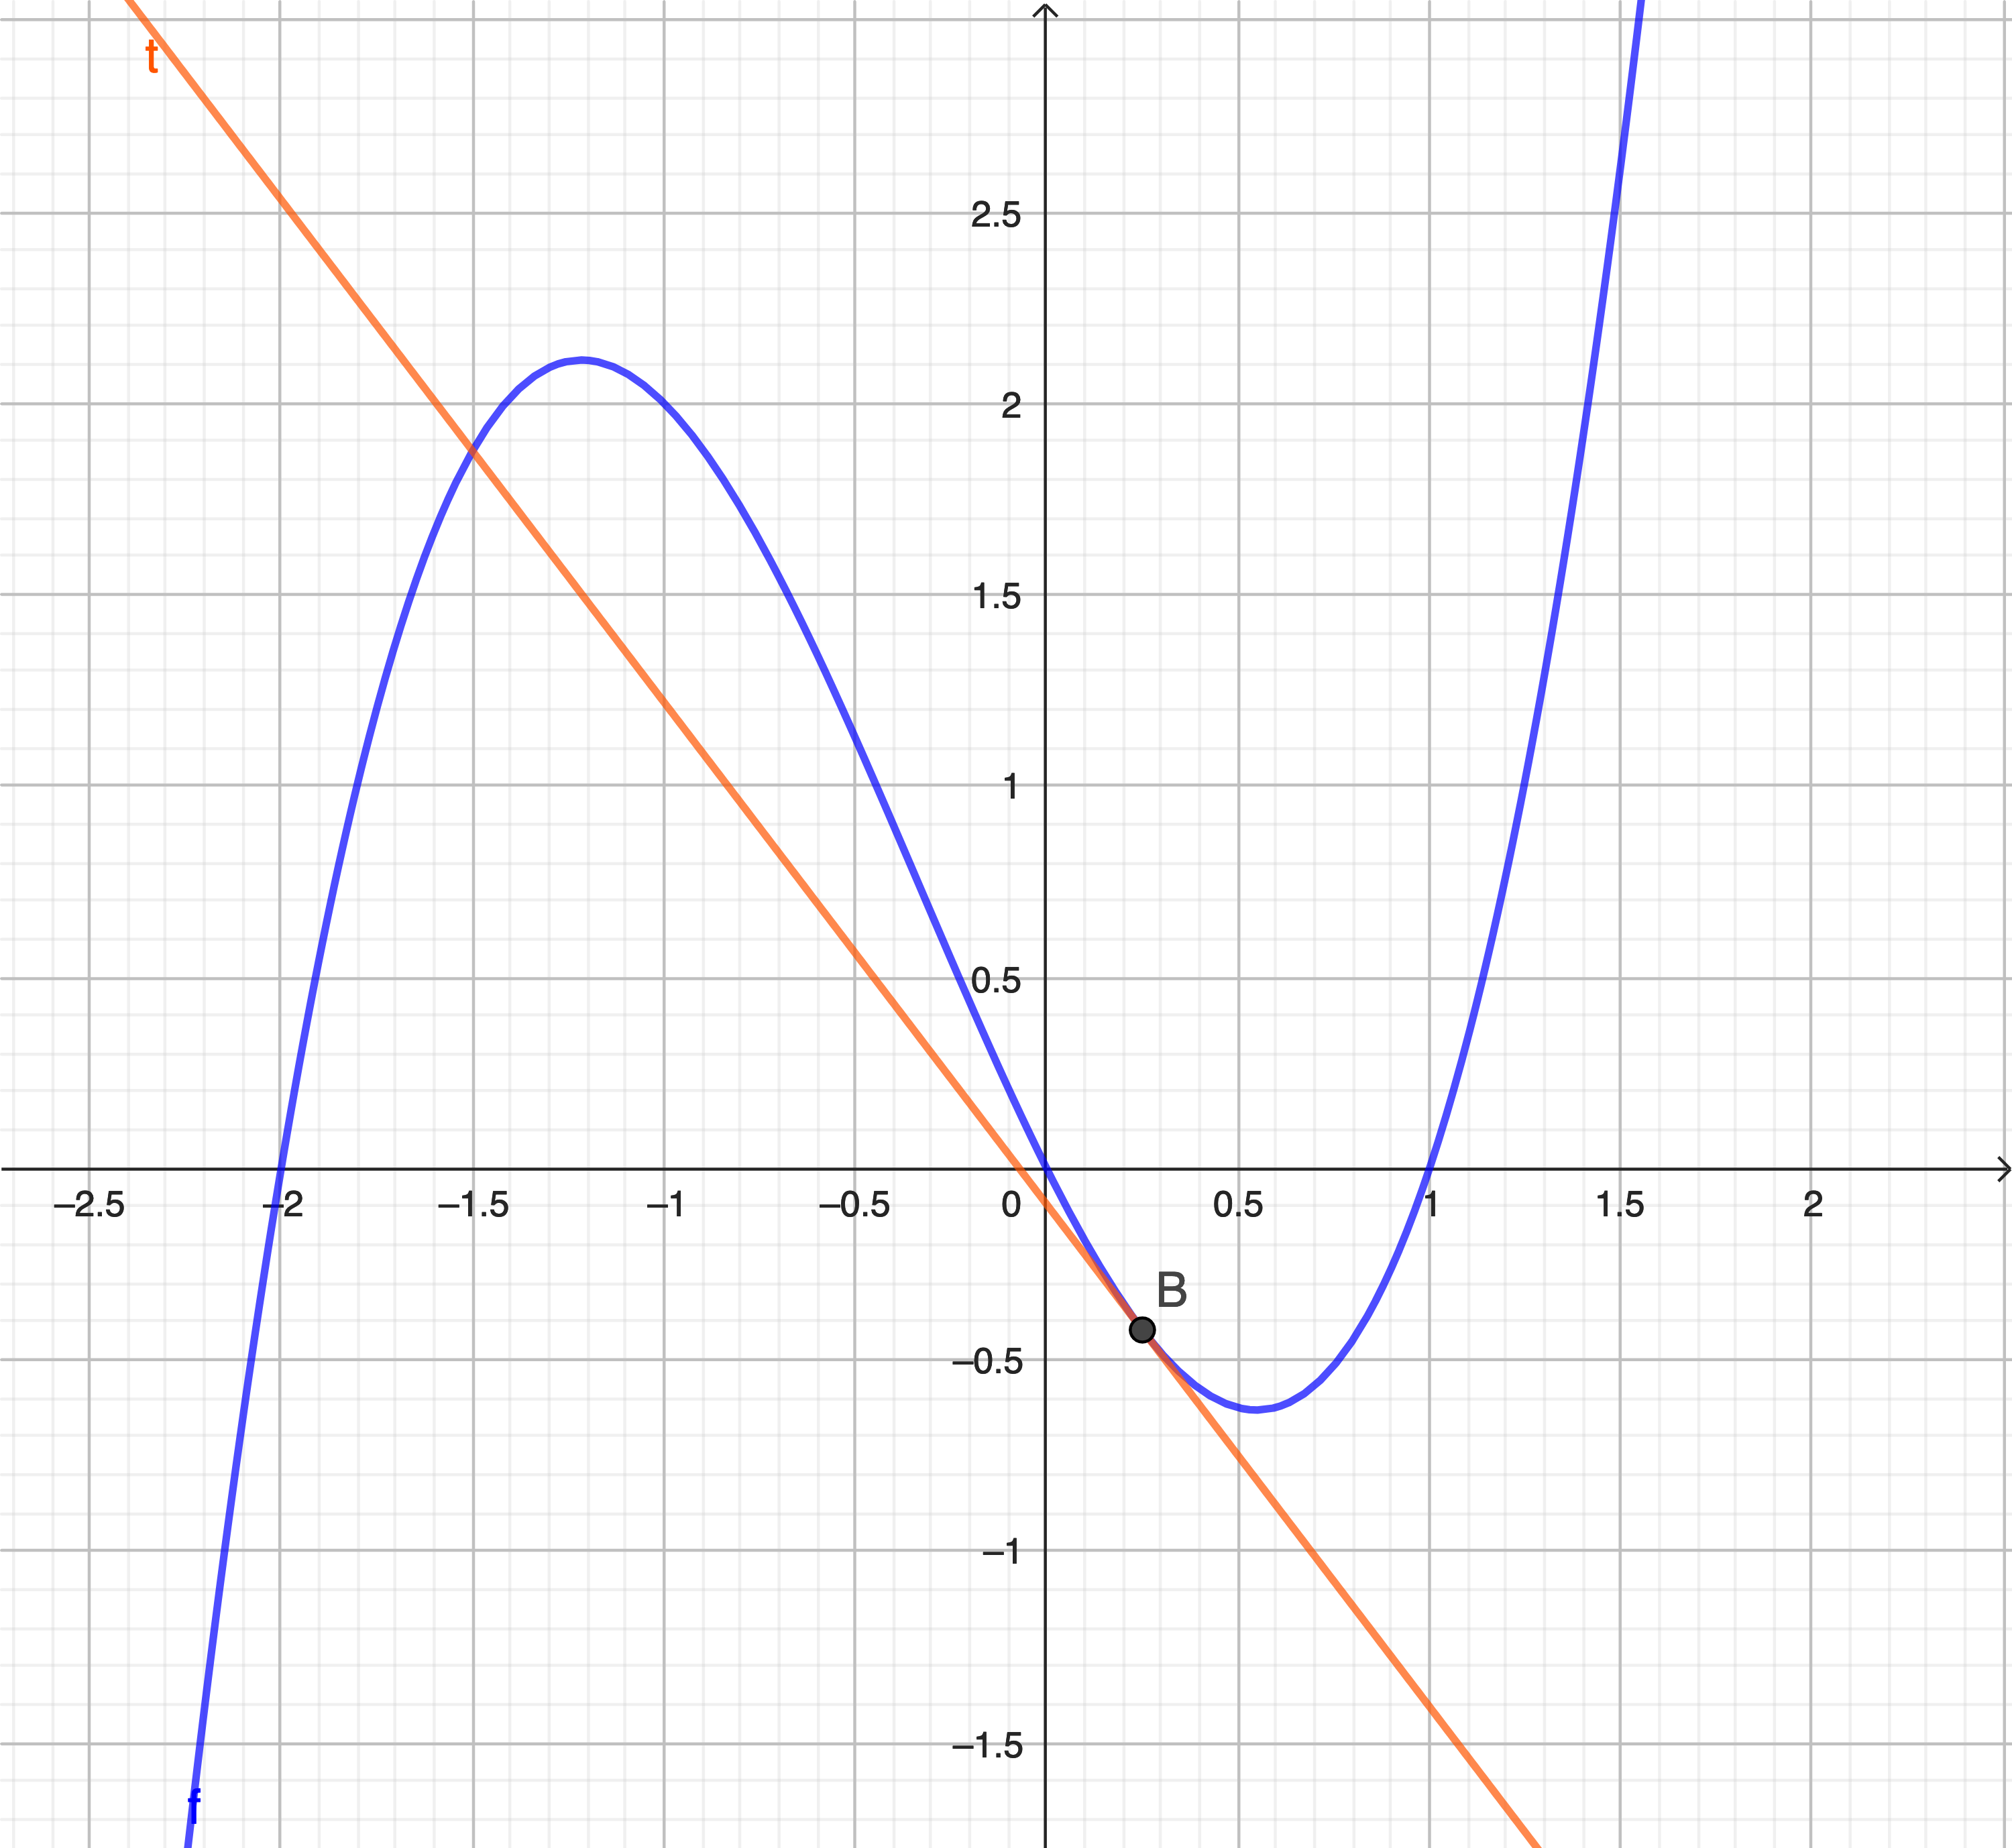
\includegraphics[scale = 1.3]{media/tangenteDef.png}
\end{center}
 
Nicht nur Geraden und Graphen können sich berühren, auch Graphen und andere Graphen:
\begin{definition}{Graphen, die sich berühren}{}
    Wenn für zwei Funktionen $f$ und $g$ gilt
    $$f'(x_0)=g'(x_0) \qquad \text{und} \qquad f(x_0)=g(x_0)$$
    Dann sagt man, dass sich die beiden Funktionsgraphen  an der Stelle $x_0$ \emph{berühren}.
\end{definition}

Bemerkung: Wenn sich zwei Graphen berühren, haben sie im Berührungspunkt eine gemeinsame Tangente.

\begin{center}
    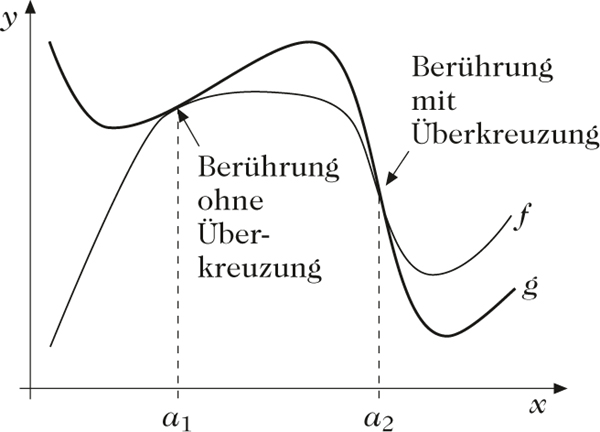
\includegraphics[scale=0.2]{media/Beruhrung-zweier-Funktionen-I11.jpg}
\end{center}


\clearpage
\begin{ueb}{}{}
    \begin{enumerate}
        \item Zeigen Sie, dass sich die Graphen der Funktionen $f(x) = x^2-3$ und $g(x) = x^3-x-2$ an der Stelle $x=1$ berühren.
        \item Zeigen Sie, dass sich die Graphen der Funktionen $f(x) = e^{x-2}$ und $g(x) = \left(\frac{x}{2}\right)^2$ an der Stelle $x=2$ berühren. \\
        Berechnen Sie anschliessend die Nullstelle der gemeinsamen Tangente.
        \item Gegeben sind die Funktionen $f(x) = \sin(x)$ und $g(x) = c- \cos(x)$. Bestimmen Sie den Wert von $c\in \R$, sodass sich die beiden Graphen im Bereich $x\in [0, 2\pi]$ berühren.\\
        Tipp: Wenn die Gleichung für den Vergleich der Steigungen schwierig zu lösen ist, versuchen Sie beide Seiten durch $\cos(x)$ zu teilen.
    \end{enumerate}
\end{ueb}


\emph{Lösungen:}
\begin{enumerate}
    \item \dots
    \item Nullstelle der gemeinsamen Tangente: $x=1$
    \item $x= \sqrt{2}$
\end{enumerate}

























\clearpage
\subsubsection{Schnittwinkel}
\begin{LA}
    {Einführungsaufgabe zu Schnittwinkel und Senkrechtstehen}{}
    \begin{enumerate}
        \item Winkel zwischen Kurven: \newline
        Beim Wiedereintritt einer bemannten Raumkapsel muss der Winkel, in dem die Raumkapsel in die Atmosphäre eindringt, in einem ganz bestimmten Bereich liegen. Wenn die Raumkapsel zu flach auf die Atmosphäre eintrifft, prallt sie ab. Wenn der Winkel zu steil ist, verglüht sie.
        Wie misst man aber den Winkel zwischen zwei \glqq krummen\grqq{} Linien? Messen Sie den ungefähren Aufprallwinkel in der Skizze unten. 
        \begin{center}
            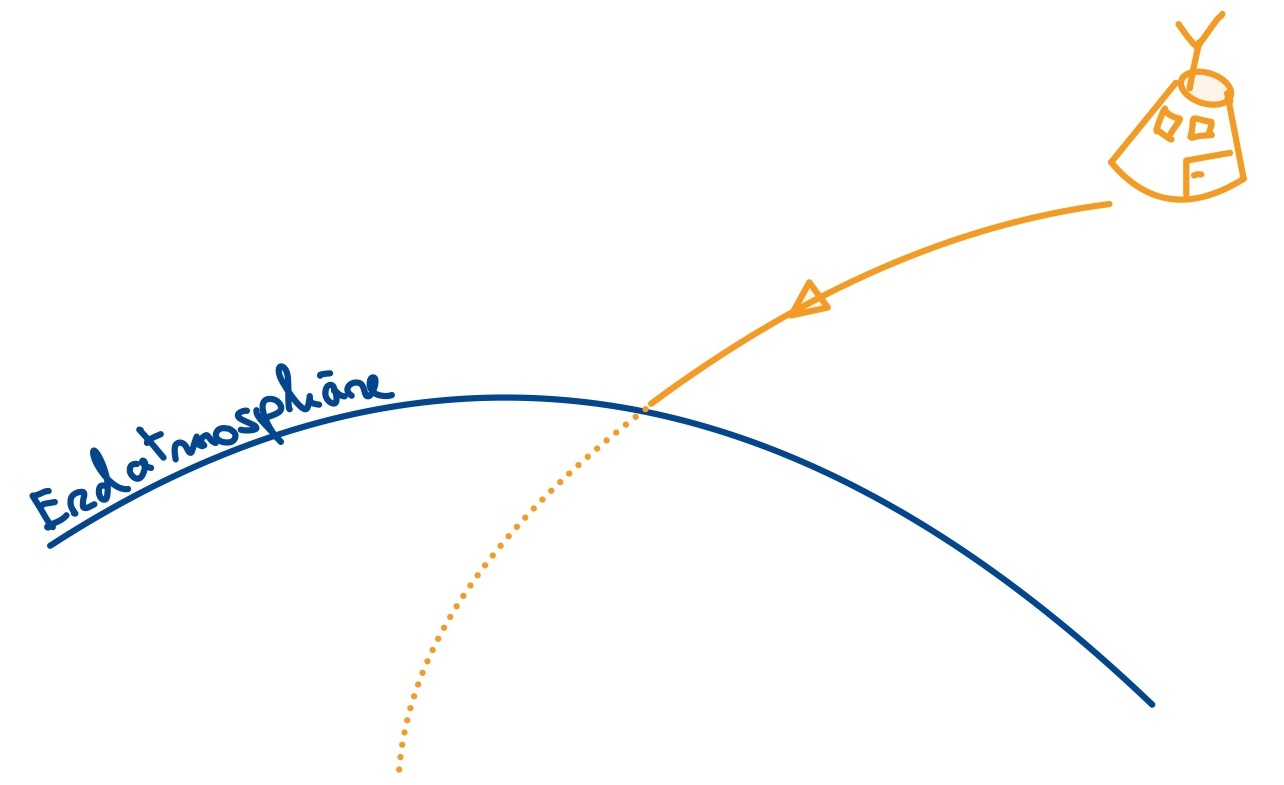
\includegraphics[width = 0.6\textwidth]{media/IntroWinkel.jpg}
        \end{center}
        \item Senkrechte Geraden: \newline
        Im Bild ist der Graph der Geraden $g: \,  y=2x$ dargestellt. Zeichnen Sie die Senkrechte zur Geraden durch den Punkt $A$. Welche Steigung hat sie? Wie erkennt man an der Steigung, ob zwei Geraden senkrecht stehen?
        \begin{center}
            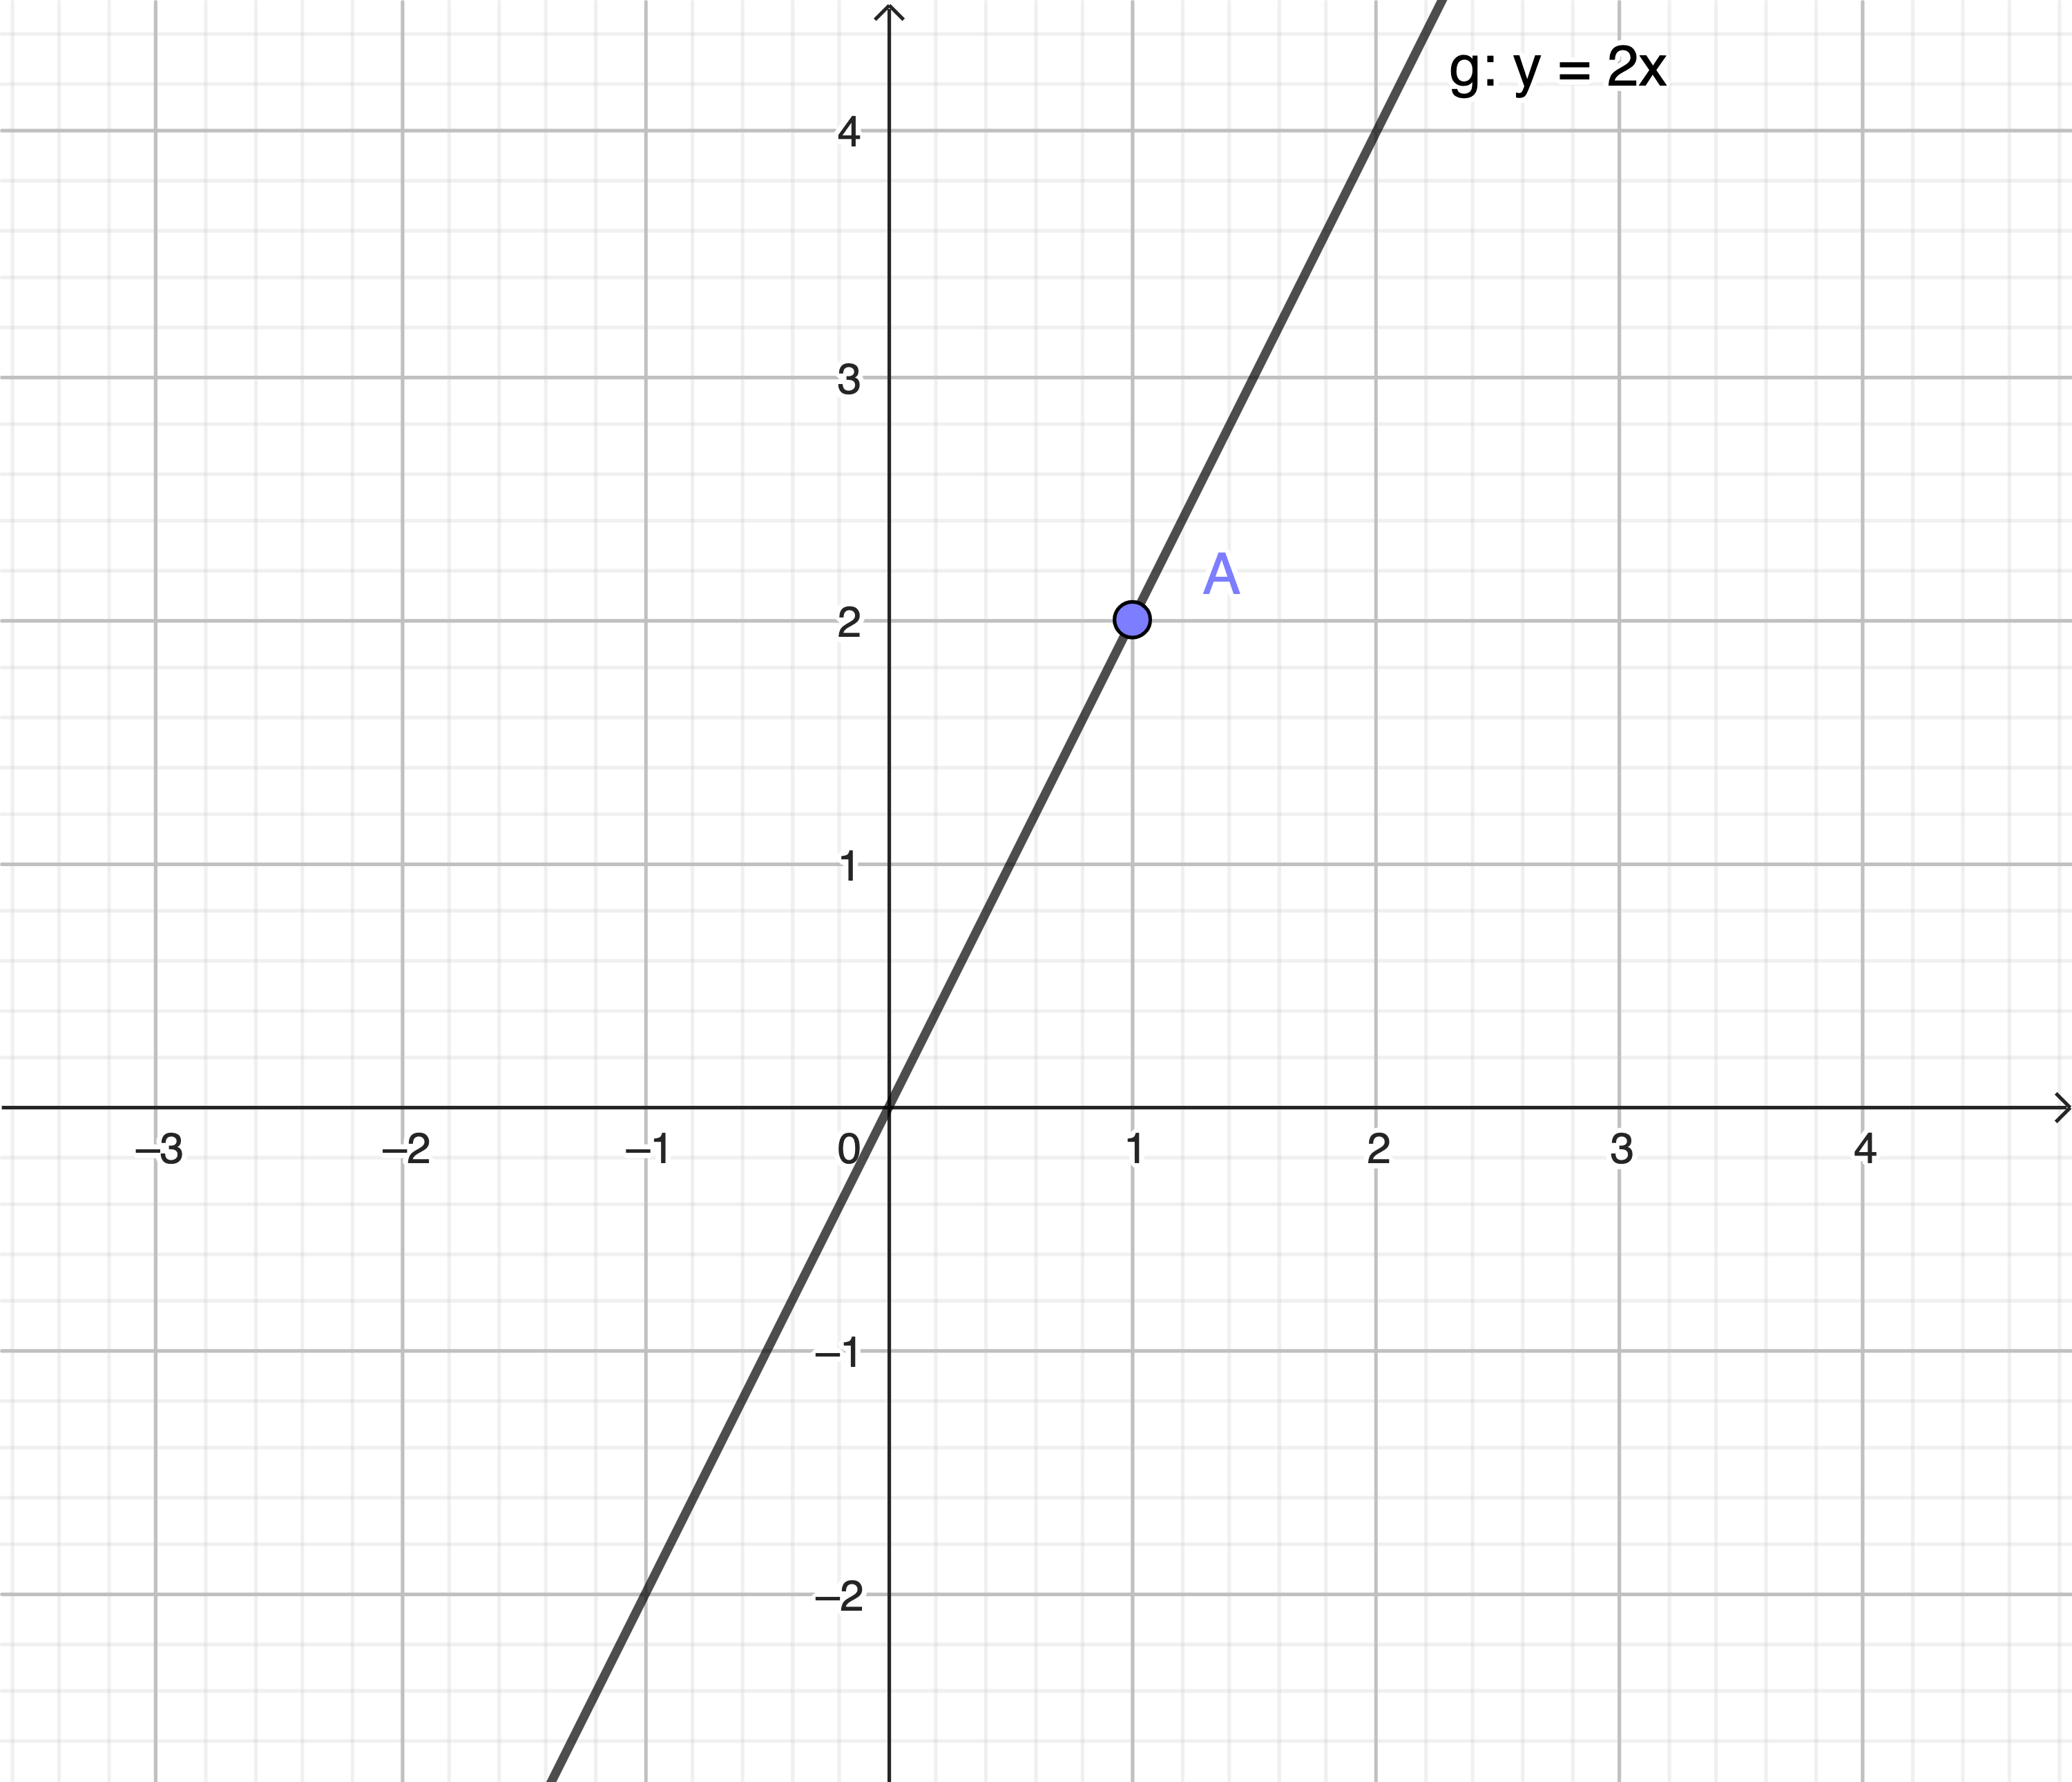
\includegraphics[width = 0.6\textwidth]{media/senkrechteGeraden.png}
        \end{center}
        \newpage
        \item Winkelberechnung: 
        \begin{enumerate}
            \item Zeichnen Sie in den Graphen der Geraden $y=2x$ oben das Steigungsdreieck mit den Ecken $(0|0), (1|0)$ und $A$.
            \item Berechnen Sie den Winkel $\alpha$ zwischen der Geraden $g$ und der $x$-Achse (Verwenden Sie dazu den Tangens!).
            \item Zeichnen Sie die Gerade $h$ durch den Ursprung mit der Steigung $a=\frac{1}{3}$. Welchen Winkel $\beta$ bildet sie mit der $x$-Achse?
            \item Welchen Winkel schliessen die beiden Geraden $g$ und $h$ ein?
        \end{enumerate}
        \item Formeln:
        \begin{enumerate}
            \item Geben Sie eine Formel an, mit der man den Winkel zwischen den beiden Geraden $g:\,   y=a_1 x+b_1$ und $h:\,  y=a_2 x+b_2$ berechnen kann.
            \item  Stimmt die Formel auch, wenn eine oder beide Steigungen negativ sind? Wieso?
        \end{enumerate} 
    \end{enumerate}
\end{LA}
\clearpage
Im Folgenden Abschnitt wird das Verfahren zur Berechnung des Schnittwinkels zwischen zwei Funktionsgraphen erklärt. Bevor damit begonnen wird, muss allerdings zuerst erklärt werden, was unter dem Winkel zwischen zwei \glqq krummen Linien\grqq{} gemeint ist:
\begin{definition}
    {Schnittwinkel}{}
    Der Schnittwinkel von zwei Kurven ist der Winkel zwischen den Kurventangenten im Schnittpunkt:
    \begin{center}
        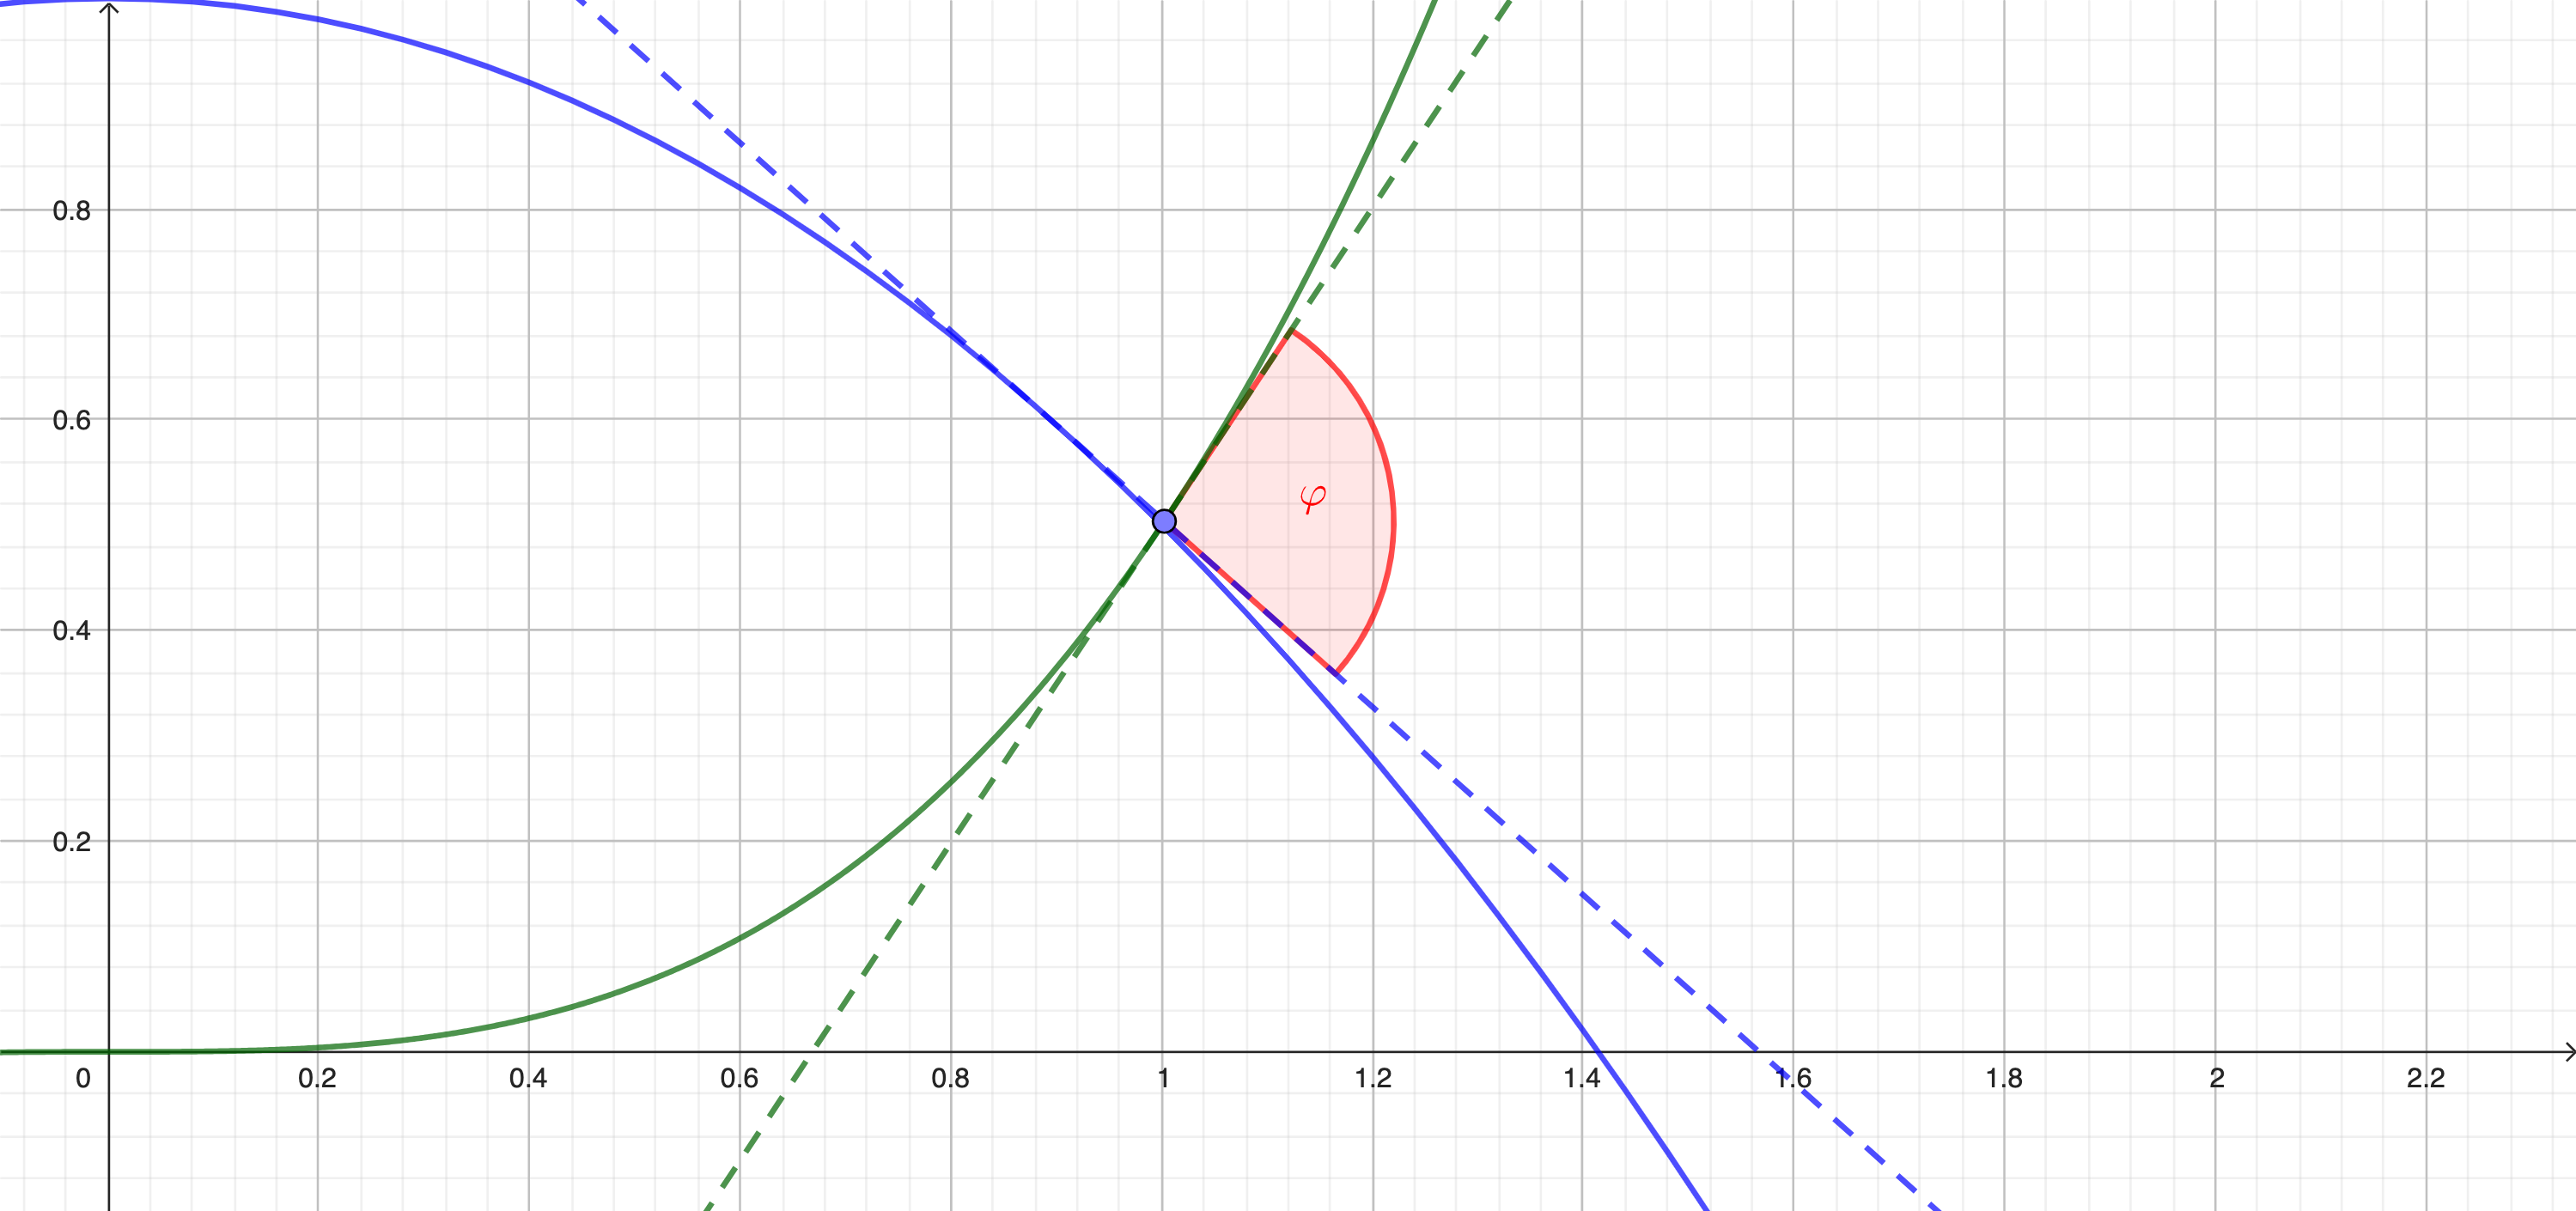
\includegraphics[width = 0.8 \textwidth]{media/WinkelZwKurven.png}
    \end{center}
\end{definition}

Als nächstes stellt sich die Frage, wie der Winkel zwischen zwei Geraden berechnet werden kann. In dem Fall, wo die eine Gerade die $x$-Achse ist, lässt sich der Winkel einfach berechnen. Betrachten Sie dazu die folgende Skizze: 
\begin{center}
    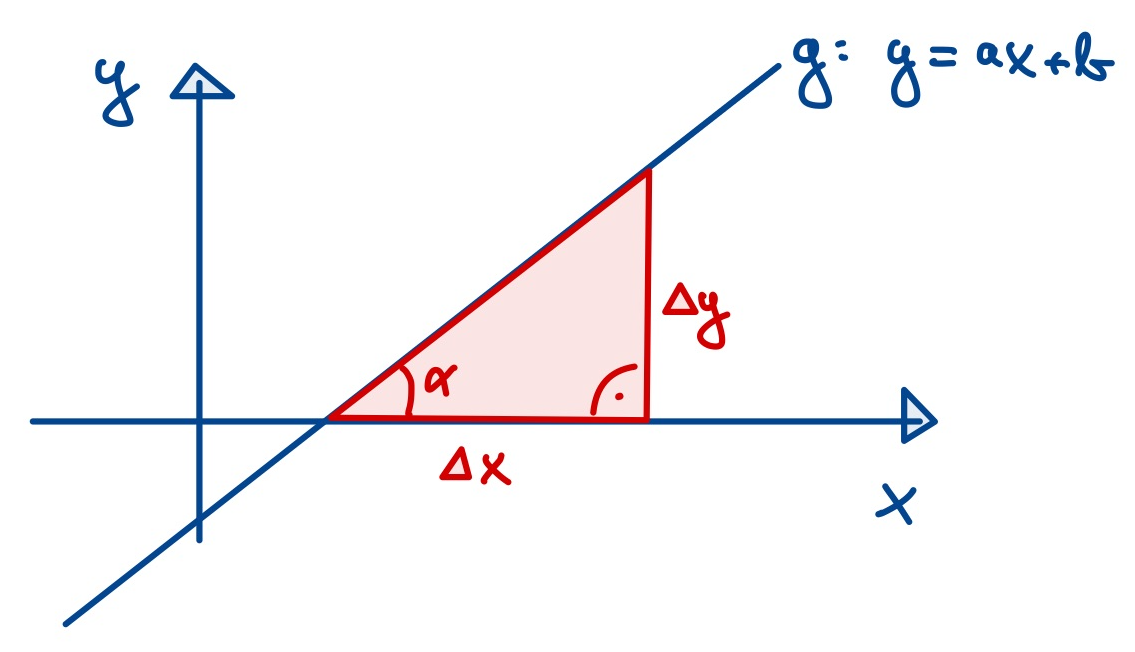
\includegraphics[width = 0.5\textwidth]{media/Winkelx-Achse.png}
\end{center}
Im markierten Steigungsdreieck gilt:
$\tan(\alpha)=\frac{\Delta y}{\Delta x}$
Das Verhältnis $\frac{\Delta y}{\Delta x}$ entspricht der Steigung $a$ der Geraden. Also
$\tan(\alpha) = a$
Damit folgt
$$\alpha = \arctan(a)$$
Im Allgemeinen kann der Winkel zwischen zwei Geraden mit folgender Überlegung berechnet werden:
\begin{center}
    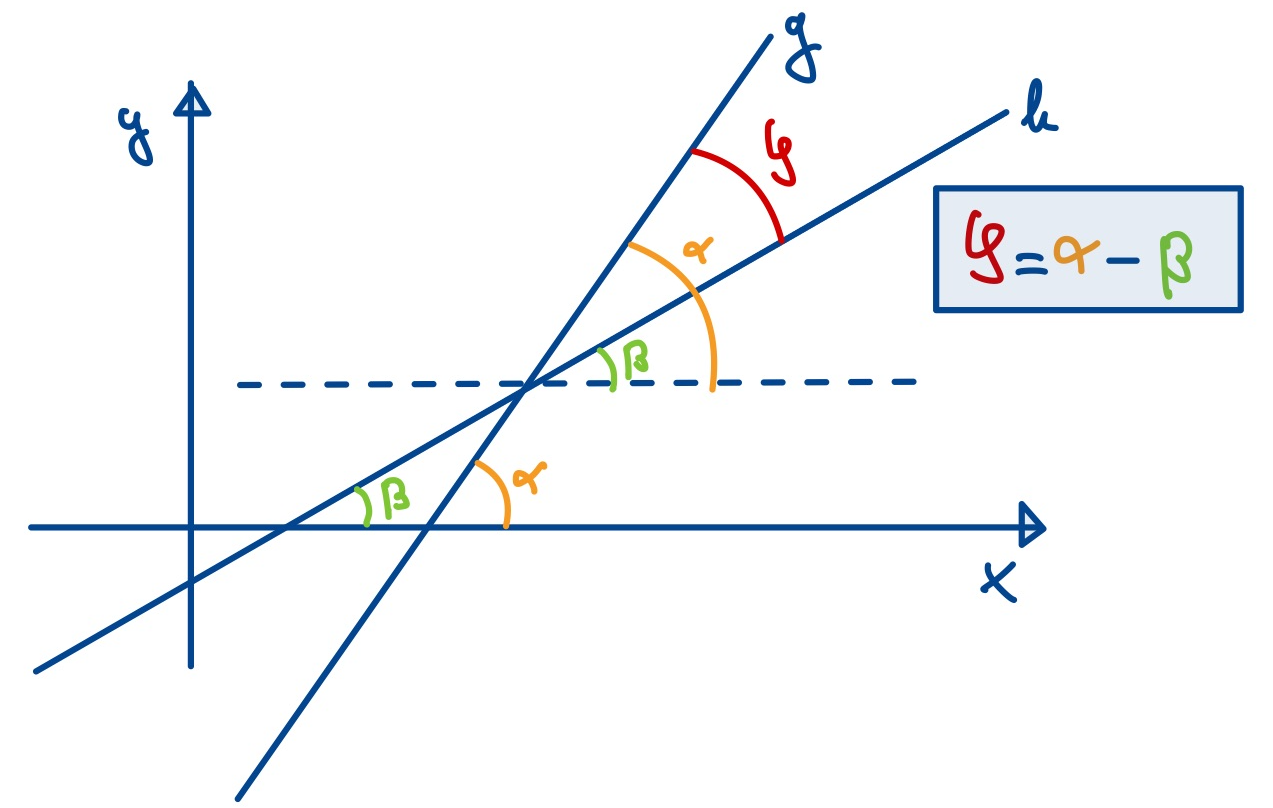
\includegraphics[width = 0.5\textwidth]{media/schnittwinkelZweiGeraden.png}
\end{center}
Zusammengefasst erhalten wir den folgenden Satz:
\begin{satz}
    {Winkelberechnungen}{}
    Der Winkel zwischen zwei Geraden $g:\,   y=a_1 x+b_1$ und $h: y=a_2 x+b_2$ ist
$$\varphi = | \arctan(a_1) - \arctan(a_2) | $$

Der Winkel zwischen den Kurven $y=f(x)$ und  $y=g(x)$, die sich an der Stelle $x_0$ schneiden, ist
$$\varphi = | \arctan(f'(x_0)) - \arctan(g'(x_0)) | $$

\end{satz}

Bemerkungen:
\begin{itemize}
    \item 	Zwei Geraden stehen genau dann senkrecht aufeinander, wenn $a_1 \cdot a_2=-1$ gilt. Entsprechend stehen zwei Kurven genau dann senkrecht aufeinander, wenn an der Schnittstelle $x_0$ gilt $f'(x_0) \cdot g'(x_0)=-1 $.
    \item Die Senkrechte einer Tangente im Berührungspunkt heisst \emph{Kurvennormale}.
    \item Die Formel von oben gilt auch im Fall, dass eine (oder beide) Steigungen negativ sind.
\end{itemize}

\begin{bsp}
    {Berechnung des Schnittwinkels}{}
    In welchem Winkel schneiden sich die Graphen von $f(x)=x^2+2x$ und $g(x)=-x^2-x$?

    % \begin{enumerate}
    %     \item Schnittstellen bestimmen:
    %     $$f(x)=g(x) \iff x^2+2x = -x^2-x \iff 2x^2+3x= 0 \iff x(2x+3) = 0 $$
    %     Die Graphen schneiden sich an den Stellen $x=0$ und $x=-\frac{3}{2}$.

    %     Im Weiteren wird nur der Winkel an der Stelle $x=0$ berechnet.
    %     \item Ableitungen
    %     \begin{align*}
    %         f'(x)=2x+2 &\Rightarrow f'(0) = 2 \\
    %         g'(x)= -2x-1 & \Rightarrow g'(0)=-1
    %     \end{align*}
    %     \item Formel für den Winkel an der Stelle $x=0$
    %     $$ \varphi = \arctan(2)-\arctan(-1) \approx 63.43^\circ -(-45^\circ) =108.43^\circ $$

    % \end{enumerate}

    \vspace*{4cm}

    \phantom{text}


    \clearpage
    \phantom{text}
    
     \vspace*{6cm}

\end{bsp}

% Speziell ist der Fall, wenn zwei Kurven sich rechtwinklig schneiden:

% \begin{satz}
%     {}{}
%     Zwei Kurven $y=f(x)$ und $y=g(x)$, die sich an der Stelle $x_0$ schneiden, stehen senkrecht aufeinander, wenn 

%     $$ g'(x_0) = - \frac{1}{f'(x_0)} $$

% \end{satz}





\begin{ueb}
    {}{}
    \begin{enumerate}
        \item
        Die Parabel \( p \) mit \( y = 2 - \frac{1}{2}x^2 \) schneidet die \( x \)-Achse im Punkt \( R \) rechts vom Ursprung. In diesem Punkt \( R \) wird die Tangente \( t \) an die Parabel \( p \) gelegt und die Normale \( n \) zur Parabel \( p \) errichtet.
        \begin{enumerate}
            \item In welchen Punkten \( T \) und \( N \) schneiden die Tangente \( t \) bzw. die Normale \( n \) die \( y \)-Achse?
            \item In welchem Punkt \( S \) schneidet die Normale \( n \) die Parabel \( p \) ein zweites Mal?
            \item In welchem Winkel schneidet die Parabel die $x$-Achse?
        \end{enumerate}
     \item
        Berechne die Schnittwinkel der folgenden Kurven

        
                \begin{enumerate}
                    \item \( k_1: y = f(x) = \cos(x), \quad k_2: y = g(x) = \sin(x), \quad 0 \leq x \leq \dfrac{\pi}{2} \). \\
                    (Tipp zur Schnittstelle: Teile die Gleichung durch $\cos(x)$)
                    \item \( k_1: y = f(x) = \dfrac{2}{x^2 + 1} \), \quad
                        \( k_2: y = g(x) = x^2 \). \\
                        (Tipp zur Schnittstelle: Substituiere $u=x^2$)
                    % \item \( y = k_1(x) = \dfrac{3 - x}{(x - 2)^2} \), \quad
                    %     \( y = k_2(x) = x - 3 \)
                    \item \( y = k_1(x) = e^{-\frac{x + 1}{2}} \), \quad
                        \( y = k_2(x) = e^{-x^2} \)
                    \item \( y = k_1(x) = \ln(x + 3) \), \quad
                        \( y = k_2(x) = \ln(7 - x) \)
                \end{enumerate}


\item Für welchen Wert des positiven Koeffizienten \( a \) schneiden sich die beiden Graphen der Funktionen
\[
f(x) = ax^2 \quad \text{und} \quad g(x) = \frac{1}{x}
\]
orthogonal, d.\,h.\ rechtwinklig?



    \end{enumerate}
\end{ueb}


\clearpage
\emph{Lösungen:}
\begin{enumerate}
    \item
    \begin{enumerate}
        \item \( T = (0, 4), \quad N = (0, -1) \)
        \item \( S = (-3, -2.5) \)
        \item \( \varphi \approx 63.4^\circ \)
    \end{enumerate}

    \item
    \begin{enumerate}
        \item \( \varphi \approx 70.5^\circ \)
        \item \( \varphi_1 = \varphi_2  \approx 71.6^\circ \)
        \item \( \varphi_1 \approx 25.9^\circ \quad \varphi_2  \approx 59.2^\circ\)
        \item \( \varphi \approx 22.6^\circ \)
    \end{enumerate}

    \item \( a = \dfrac{1}{2} \sqrt[4]{2} \approx 0.6\)
\end{enumerate}

